\documentclass[11pt]{llncs2e/llncs}
\usepackage{amsmath,amscd,amsfonts,amssymb,mathrsfs}
\usepackage{rotating}
\usepackage[english]{babel}
%\usepackage[latin1]{inputenc} % si WINDOWS
%\usepackage[utf8]{inputenc} % si LINUX
%\usepackage[T1]{fontenc}

\usepackage{graphicx}
%\usepackage[xetex]{graphicx}
\usepackage{tikz} 
  \usetikzlibrary{chains}
    \usetikzlibrary{positioning}
\definecolor{mycolor}{RGB}{8,108,131}

\usepackage{slashbox}
\usepackage{multirow}

\addtolength{\hoffset}{-1cm}
\addtolength{\textwidth}{2cm} 
\addtolength{\voffset}{-2cm} 
\addtolength{\textheight}{4cm} 


\usepackage{url}
\usepackage{algorithm}

%\usepackage{algorithm}
\usepackage[noend]{algorithmic}
%\usepackage{varioref}

\pagestyle{plain}

%\usepackage{array}
%\usepackage{amsmath}
%\usepackage{amsfonts}
%\usepackage{amssymb}

\usepackage{xcolor}
\usepackage{color}
\usepackage{hyperref}
\hypersetup{
    bookmarks=true,         % show bookmarks bar?
%    unicode=false,          % non-Latin characters in Acrobat's bookmarks
%    pdftoolbar=true,        % show Acrobat's toolbar?
%    pdfmenubar=true,        % show Acrobat's menu?
%    pdffitwindow=false,     % window fit to page when opened
%    pdfstartview={FitH},    % fits the width of the page to the window
    pdftitle={CoinCurves}, 
  % title
%    pdfauthor={Renaud Dubois and Aurore Guillevic and Marine Sengelin Le Breton}     % author
%    pdfsubject={Subject},   % subject of the document
%    pdfcreator={Creator},   % creator of the document
%    pdfproducer={Producer}, % producer of the document
%    pdfkeywords={keywords}, % list of keywords
%    pdfnewwindow=true,      % links in new window
%    colorlinks=true,        % false: boxed links; true: colored links
%    linkcolor=c12,          % color of internal links
%    citecolor=c25,          % color of links to bibliography
%    filecolor=c18,          % color of file links
%    urlcolor=c13            % color of external links
}

% \usepackage{tikz}
% \usetikzlibrary{shapes,arrows}
% \usetikzlibrary{positioning}
% \usetikzlibrary{positioning,shadows,backgrounds}
% \usetikzlibrary{trees}

\newcommand{\gray}[1]{\textcolor{gray}{#1}}
\newcommand{\lightgray}[1]{\textcolor{lightgray}{#1}}


\DeclareMathOperator*{\cat}{\parallel}
\newcommand{\hw}{\operatorname{\mathsf{H}}}
\newcommand{\pr}{\operatorname{P}}
\newcommand{\esp}{\operatorname{E}}
\newcommand{\cor}{\operatorname{Cor}}
\newcommand{\abs}[1]{\left|#1\right|}
\newcommand{\sep}{\;\vert\;}
\newcommand{\I}{\operatorname{I}}
\newcommand{\C}{\operatorname{\mathscr{C}}}
\newcommand{\X}{\mathfrak{S}}
\newcommand{\Y}{\mathfrak{S}'}

\newcommand{\NN}{\mathbb{N}}
\newcommand{\ZZ}{\mathbb{Z}}
\newcommand{\CC}{\mathbb{C}}

\newcommand{\G}{\mathbb{G}}

\newcommand{\PO}{\mathcal{O}}
\newcommand{\F}{{\mathbb{F}\!}}
\newcommand{\Fp}{\F_p}
\newcommand{\Fpk}{\F_{p^k}}
\newcommand{\Fr}{\F_r}

\newcommand{\Fq}{\F_q}

\newcommand{\PK}{\mbox{PK}}
\newcommand{\SK}{\mbox{SK}}

\newcommand{\added}[1]{\textbf{#1}}
\usepackage[normalem]{ulem}
%\sout{Texte a barrer}
%\xout{Texte a hachurer}
%\uwave{Texte a souligner par une vaguelette}
\newcommand{\removed}[1]{\sout{#1}}

% renaud.dubois@wanadoo.fr,guillevi@di.ens.fr,marine.sengelin@gmail.com

\begin{document}
\title{Cryptographic Toolbox for Privacy Preserving with Applications to Self Sovereignty}
 
   \author{
    Renaud Dubois}
  
   \institute{
     \textregistered Ledger\\ 
     6 rue Gretry, 75002 Paris -- France\\
     firstname.lastname@ledger.fr
   }


\maketitle

%%%%%%%%%%%%%%%%%%%%%%%%%%%%%%%%%%%%%%%%%%%%%%%%%%%%%%%%%%%%%%%%%%%%%%%%%%%%%%%%
%%%%%%%%%%%%%%%%%%%%%%%%%%%%%%%%%%%%%%%%%%%%%%%%%%%%%%%%%%%%%%%%%%%%%%%%%%%%%%%%

\begin{abstract}

Self-sovereign identity (SSI) is an approach to digital identity that gives individuals control of their digital identities. In the Web3 framework, this {\bf D}ecentralized {\bf Id}entity is referred as DId \cite{W3CDId21}. In the litterature, the dedicated Cryptographic solution is referred as Anonymous Credentials (AC) \cite{CL02}, \cite{CL04}. It is a complex protocol that requires the use of several Privacy-Preserving protocols. 
The aim of this memo is to provide an overview of existing DIDs frameworks and the underlying cryptographic mechanisms in order to give an input to reflexion about how SSI could benefit to Web3 and be enforced by Ledger products and solution. 

{\bf keywords:}{  Decentralized Idenfiers,  Credential, Zero knowledge, Cryptographic Commitments}
\end{abstract}

%%%%%%%%%%%%%%%%%%%%%%%%%%%%%%%%%%%%%%%%%%%%%%%%%%%%%%%%%%%%%%%%%%%%%%%%%%%%%%%%
%%%%%%%%%%%%%%%%%%%%%%%%%%%%%%%%%%%%%%%%%%%%%%%%%%%%%%%%%%%%%%%%%%%%%%%%%%%%%%%%
%%%%%%%%%%%%%%%%%%%%%%%%%%%%%%%%%%%%%%%%%%%%%%%%%%%%%%%%%%%%%%%%%%%%%%%%%%%%%%%%
%%%%%%%%%%%%%%%%%%%%%%%%%%%%%%%%%%%%%%%%%%%%%%%%%%%%%%%%%%%%%%%%%%%%%%%%%%%%%%%%
\section*{Introduction}

\subsubsection{Decentralized Idenfiers.}

Self Sovereign Identity (SSI) : is a paradigm shift from centralized and trusted Credential issuing to a  ‘user-centric’ management of the identity. According to \cite{W3CDId21}, Decentralized identifiers (DIDs) are a new type of identifier that enables verifiable, decentralized digital identity. A DID refers to any subject (e.g., a person, organization, thing, data model, abstract entity, etc.) as determined by the controller of the DID. In contrast to typical, federated identifiers, DIDs have been designed so that they may be decoupled from centralized registries, identity providers, and certificate authorities. Specifically, while other parties might be used to help enable the discovery of information related to a DID, the design enables the controller of a DID to prove control over it without requiring permission from any other party. DIDs are URIs that associate a DID subject with a DID document allowing trustable interactions associated with that subject.

\subsubsection{Anonymous Credentials.}


In traditional electronical authentication,  user identities are readily available to service providers. These latter can exchange collected data about any particular user among themselves. Anonymous credentials aims at mitigating such privacy breaches and giving the
user  control over his data. Informally, as explained in \cite{DBLP:conf/crypto/BaumBCPGL18}, a user acts
under an arbitrary number of unlinkable pseudonyms rather than under his identity.
In anonymous credentials, these access rights are described by attributes. A service provider can issue a credential to a user, which is parameterized with attributes. These attributes can, for example,
encode access rights to a service or some user data. The user can then prove possession
of a credential to the same or to other service providers in a privacy-preserving way.
This process is called showing a credential.


The first efficient realization of anonymous credentials was first issued by Carmenish in \cite{CL02} and \cite{CL04} which demonstrated how to build such protocol using the following primitives:
\begin{itemize}
 \item a commitment scheme (the analogue of digital envelop),
 \item a signature scheme,
 \item an efficient signature scheme (a protocol to obtain a signature on a commited value without revealing the value to the signer),
 \item a zero knowledge proof of knowledge (ZKPoK, NIZKP).
\end{itemize}
The three laters are the real algorithmic stake because they are the major bottleneck.

\begin{figure}
 \begin{center} 
\input{figs/cryptostack}
 \caption{The cryptographic stack for AC construction}
 \label{fig-cryptostack}
 \end{center}
 \end{figure} 
 
\subsubsection{Contributions}
The efficiency of the design of ZKP and efficient schemes relies on the cunning imbrication of the commitment and signatures with specific properties (structure preserving, use of homomorphic additive properties, etc.). This note tries to give an overview of those imbrications and the evolution of the state of the art to its current shape. We acknowledge the previous work of   \cite{PrimforW3} and  section D.5.2.1 of Prometheus project \cite{Prom} as a starting point of the redaction  of this note and our comprehension. The note is structured as follows:
\begin{itemize}
 \item the first section gives an overview of the cryptographic primitives used for AC constructions (figure \ref{fig-cryptostack}),
 \item the second section provides a state of the art of existing Anonymous Credentials in the wild with fair Comparizon,
 \item the last section provides a survey of existing project and applications in \textregistered Ledger that would benefit of such privacy preserving mechanisms.
\end{itemize}
The note has a minor contribution in the generalization of functional commitment to linear function described in \cite{Libert16} to ideal Universal commitment. Unfortunately the practical (in term of complexities) commited functions are however quite limited.
 
%%%%%%%%%%%%%%%%%%%%%%%%%%%%%%%%%%%%%%%%%%%%%%%%%%%%%%%%%%%%%%%%%%%%%%%%%%%%%%%%
%%%%%%%%%%%%%%%%%%%%%%%%%%%%%%%%%%%%%%%%%%%%%%%%%%%%%%%%%%%%%%%%%%%%%%%%%%%%%%%%
%%%%%%%%%%%%%%%%%%%%%%%%%%%%%%%%%%%%%%%%%%%%%%%%%%%%%%%%%%%%%%%%%%%%%%%%%%%%%%%%
%%%%%%%%%%%%%%%%%%%%%%%%%%%%%%%%%%%%%%%%%%%%%%%%%%%%%%%%%%%%%%%%%%%%%%%%%%%%%%%%
\section{State of the Art}

\subsection{Commitments}

\subsubsection{First examples}

\vskip+0.1cm

\begin{figure}
 \begin{center} 
\input{figs/commitment.tickz}
 \caption{Evolution of Commitment schemes}
 \end{center}
 \end{figure} 
 
 A commitment scheme emulates a publicly observed sealed envelope; it
allows a party to commit to a message $m$ so that this message is not revealed until a
later moment when the commitment is opened and the receiver gets convinced that the
message was indeed m. Two important security properties of commitment schemes are
called {\bf hiding} and {\bf binding}. The first property requires that no information about the committed message is revealed to an observer. The second property means that the committing party cannot alter the message after committing to it. 
The first well known way to commit is to commit to the hash of a value. In this trivial scheme, the value of the envelope $m$ is commited though its hash $h(m)$. It is possible for the Prover to proove the knwoledge of $m$ by providing its commitment. This solution is classically used in online Password authentication, which can be considered as a zero knowledge proof of the value $m$. In \cite{Pedersen91}, the author describes a commitment scheme with {\bf homorphic additive property}. Pedersen Vector Commitment is a direct corollary of this additive feature. He also provides the first description of a Verifiable Secret Sharing Scheme, which use the proposed commitment as a tool to provide a verification aspect to the well known Shamir Secret Sharing Scheme \cite{Shamir79} (which is in fact a diverted way to use a Reed Solomon Code). This scheme introduce the idea of an ``{\bf Opening function}'', formalized later on. Indeed while commiting to $x_1$ and $x_2$, it is possible to reveal later the value $x_1+x_2$, without revealing separately the $x_i$. This property is used in Monero to hide transaction amount with blinding factors. It has also been used in BulletProof for a {\bf range proof system}. {\it TODO : hunt for more Perdersen Commitment uses in the litterature}.
  

 \begin{figure}[h!]
 \fbox{\parbox{\textwidth}{
{\bf Pedersen Commitment}
 \begin{itemize} 
  \item $Setup(1^\kappa,t)$ :  $<G,Q> \leftarrow^\$ E(F_p) $ 
  \item $Commit(x,r)$ :  ${\cal{C}}(x,r)=xG+rQ$  
  \item $Addition: \sum {\cal C}(x_i,r_i)$ :  ${\cal{C}}(\sum x_i,\sum r_i)$  
  
 \end{itemize}
 }}

 \fbox{\parbox{\textwidth}{
{\bf Pedersen Vector Commitment}
 \begin{itemize} 
  \item $Setup(1^\kappa,t)$ :  $<G_1, \ldots, G_n,Q> \leftarrow^\$ E(F_p) $ 
  \item $Commit(\vec{x},r)$ :  ${\cal{C}}(\vec{x},r)=\sum x_iG_i+rQ$  
 \end{itemize}
 }}
 \caption{Pedersen Commitments \cite{Pedersen91}}
 \end{figure}
 
 \subsubsection{Definitions.} Now that some insight with basic constructions have been provided, the definition of a Universal Commitment is given. It appears as a natural extension of the Functional Linear Commitment of \cite{Libert16} to any function. 
  
 \begin{figure}[h!]
 \fbox{\parbox{\textwidth}{
{\bf Ideal Universal Commitment}
 \begin{itemize} 
  \item $Setup(1^\kappa,t)$ : takes security parameter $\kappa$ and additional parameters $t$ then output an algebraic structure, optionally some $<P_k,S_k>$ elements.
  \item $Commit(S_K,r)$ : outputs commitment $\cal{C}$ to element $r$ and (optionally) auxiliary information $\tt{aux}$
  \item $Open(S_K, r)$ output element r
  \item $Witness(S_K, r, i )$ output $<i, f(i,r), w_i>$ where $w_i$ is a witness of the evaluation of $f$ in $i$ relatively to the commited element $r$.
  \item $VerifyOpen(S_K, {\cal{C}}, i, r, f(i,r))$
  \item $VerifyEval(P_K, i, f(i,r), w_i)$ 
 \end{itemize}
 }}
\caption{Ideal Universal Commitments Formalization (this note)}
 \end{figure}
 
\begin{table}
\begin{center}
 \begin{tabular}{ |c| c|c|c|c|}
  \hline
  Scheme & Commit & Open & Witness & f \\
  \hline
 \end{tabular}
 \end{center}
 \caption{Instanciation of known commitment schemes in the Universal Commitment framework (TBD)}
\end{table}

\subsubsection{Polynomial Commitment}
 
 Polynomial commitments are used to provide exact range proof. The idea is to commit a Polynomial that is evaluated to $0$ in all elements of the interval. It is done by commiting a polynomial P=($\prod x_i-a_i$)Q where $Q$ is used for security.
  
 \begin{figure}[h!] 
 \fbox{\parbox{\textwidth}{
{\bf Polynomial Commitment}
 
 \begin{itemize} 
  \item (Trusted) Setup : $(g, g^\alpha, g^{\alpha^2}, \ldots, g^{\alpha^d}), (h, h^\alpha, h^{\alpha^2}, \ldots, h^{\alpha^d}$) 
  \item Com(p,r) : $(\prod_{j=0}^d (h^{\alpha^j})^{p_j}).(\prod_{j=0}^d (g^{\alpha^j})^{r_j})$, $p(x)=\sum p_jx^j, r(x)=\sum r_jx^j$
  \item Open: output $(p,r)$
  \item VerifyPoly : output ${\cal{C}}\stackrel{?}{=}g^{p(\alpha)}.h^{r(\alpha)}$
  \item Witness : 
  \item VerifyEval : 
 \end{itemize}
 }}
 
\caption{Polynomial Commitment \cite{Kate10}}
 \end{figure}
 
 \subsubsection{Applications}
 
 
\begin{table}
\begin{center}
 \begin{tabular}{ |c| c|c|c|c|}
  \hline
  Scheme & Required for & Description \\
  \hline\hline
  Pedersen & VSS& Verifiable Secret Sharing\\
           & Monero & Transaction amount hiding \\
           & BulletProof & Range Proof \\
           & Credentials & \cite{LCKO21}, \cite{ElkhiyaouiCA21} \\
  \hline
  Polynomial C. & eVSS& Strongly Verifiable Secret Sharing \\
                & & Range Proof\\
                & & Credentials \\
                & & Zk-Snark \\
  \hline
  Functional Linear & & \\
  \hline
  
  \hline
 \end{tabular}
 \end{center}
 \caption{protocols build on top of described commitments schemes}
 \label{tab-usecommit}
\end{table}
 
\subsection{Efficient Signatures}

\subsubsection{Groth Signature}
Groth signature \cite{SigGroth} is a structure-preserving signature that sign vectors of group elements.

\subsection{Zero knowledge Proofs}

\subsubsection{LegoSnark: gadget for Commitments}



\begin{table}
\begin{center}
 \begin{tabular}{ |c| c|c|c|c|}
  \hline
  Scheme & Required for & Description \\
  \hline\hline
  Groth16  & Tornado Nova & Transaction hiding (Mixer)\\
           & Zcash v1& Coin ownership\\
  \hline
  Stark && \\
  \hline
  
  \hline
  
 \end{tabular}
 \end{center}
 \caption{protocols build on top of ZKP schemes}
 \label{tab-usecommit}
\end{table}
 
%%%%%%%%%%%%%%%%%%%%%%%%%%%%%%%%%%%%%%%%%%%%%%%%%%%%%%%%%%%%%%%%%%%%%%%%%%%%%%%%
%%%%%%%%%%%%%%%%%%%%%%%%%%%%%%%%%%%%%%%%%%%%%%%%%%%%%%%%%%%%%%%%%%%%%%%%%%%%%%%%
%%%%%%%%%%%%%%%%%%%%%%%%%%%%%%%%%%%%%%%%%%%%%%%%%%%%%%%%%%%%%%%%%%%%%%%%%%%%%%%%
%%%%%%%%%%%%%%%%%%%%%%%%%%%%%%%%%%%%%%%%%%%%%%%%%%%%%%%%%%%%%%%%%%%%%%%%%%%%%%%%
\section{Anonymous Credentials/DIds}

This section describes some existing frameworks with pointers to the underlying cryptographic mechanisms. The last subsection highlight a construction providing a decentralized approach.

\subsection{Existing SSI}

\begin{table}[h!]
\begin{center}
\begin{tabular}{|c|c|c|c|c|c|c|}
\hline
 &\cite{ElkhiyaouiCA21}&\cite{LCKO21} & Sovrin \cite{Sovrin}& IPv8& YL20& Uport \\
 \hline
Control &\checkmark &\checkmark &\checkmark &\checkmark &\checkmark &\checkmark  \\
\hline
Data Minimization &\checkmark &\checkmark &\checkmark &\checkmark &\checkmark & $\times$\\
\hline
Commitment Type &&&&&&\\
\hline
Signature Type &\cite{SigGroth}&&&&&\\
\hline
ZKP type &\cite{EG14} &\cite{Groth16} &\cite{CL02} & \cite{CL02}+\cite{PengB10}& & -\\
\hline
Issuer Anonymity Optimization& \checkmark & $\times$ &$\times$&$\times$&$\times$&$\times$\\
\hline 

\end{tabular}
\caption{Comparizon of existing DIds (completed from\cite{LCKO21})}
\end{center}
\end{table}

\begin{table}[h!]
\begin{center}
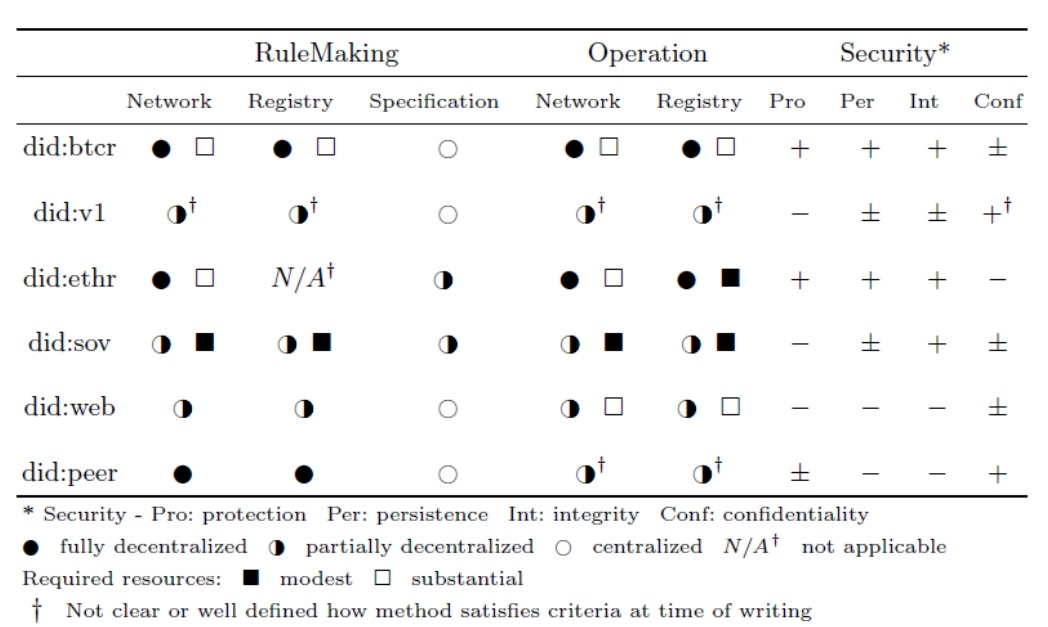
\includegraphics[width=14cm]{figs/Dids.jpg}
\caption{Comparizon of existing DIds (source : \cite{MGG18})} 
\end{center}
\end{table}

\subsection{A multi-issuer scheme}


%%%%%%%%%%%%%%%%%%%%%%%%%%%%%%%%%%%%%%%%%%%%%%%%%%%%%%%%%%%%%%%%%%%%%%%%%%%%%%%%
%%%%%%%%%%%%%%%%%%%%%%%%%%%%%%%%%%%%%%%%%%%%%%%%%%%%%%%%%%%%%%%%%%%%%%%%%%%%%%%%
%%%%%%%%%%%%%%%%%%%%%%%%%%%%%%%%%%%%%%%%%%%%%%%%%%%%%%%%%%%%%%%%%%%%%%%%%%%%%%%%
\section{Applications for Ledgers}

In this section we provide a list of Ledgers services which could benefit to an improvment of the privacy using some element of the ``toolbox''.

\subsubsection{Endorsement.} During Ledger endorsement of a Nano device, the public key is send to the BackEnd, then a ``challenge-response'' between Ledger services and Nano is performed. Using a Zero-knowledge proof instead of sending the public key would reduce the information that Ledger could store about links between a device and a host (smartphone or labtop). This could be achieved using a Group Signatures as described in this document instead. The backend only learns that it is indeed a Nano that is connecting to the Ledger Live application, without further information.


\subsubsection{Protect.} In Protect, the seed element (input to the BIP32 protocol, the core of all user security) is stored via a threshold mechanism which is a VSS (verifiable Secret Sharing scheme) which was designed by Pedersen. While 

\subsubsection{Device ID: Airdrop} One of the application of the Device Identifier (which is a very risky initiative in term of Privacy) is to perform Airdrops to the owner of nanos. 

\subsubsection{DIds resolution}


\begin{table}
 \begin{center}
  \begin{tabular}{|c|c|c|}
   \hline
   Issue Name & Description & \# (Link) \\
   \hline
   Computational Delegation of pairings & Hybrid Architecture for efficient Nano PBC&\\
   \hline
   Strongly verifiable secret sharing& eVSS for Protect &\\
   \hline
   Musig2 &  Schnorr Multisignature& \\
   \hline
   Nano with Group Signature endorsement &  Group signature for Ledger endorsement& \href{https://github.com/LedgerHQ/innovation/issues/31}{31}\\
   \hline
   Linkable signature for Airdrop & Linkable signature for Anonymous Airdrop& 30 \\
   \hline
   
  \end{tabular}

 \end{center}
\caption{Innovation issues related to Privacy Preserving}
\end{table}

%%%%%%%%%%%%%%%%%%%%%%%%%%%%%%%%%%%%%%%%%%%%%%%%%%%%%%%%%%%%%%%%%%%%%%%%%%%%%%%%
\section{Conclusion} 

In this note we provided an overview of some privacy preserving tools and principles. We also provide a non exhaustive list of applications that could immediately benefit from the described mechanisms. Most of those building blocks rely on the use of computation of pairing over elliptic curves. 




\bibliographystyle{alpha}
\bibliography{biblch}

\appendix

\section{Issues and Roadmap}



\section{Implementation of Pairings}



\subsection{Pairings used in blockchain framework}
%Barreto–Lynn–Scott BLS12, cyclotomic r(x)	12	3	0x8508c00000000001=263+258+256+251+247+246+1	Zexe, eprint 2018/962, Table 16	377	253	p2, 754	4521
%Barreto–Lynn–Scott BLS12, cyclotomic r(x)	12	3	-0xd201000000010000=-263-262-260-257-248-216	ZCash	381	255	p2, 762	4569


\subsection{Hybrid Architecture for Nano}
As a constrained device, the Implementation of pairings only on the device may 
The pairings are a bilinear map $$e:(G_1 \times G_2) \rightarrow \mathbb{F}_{p^k}, $$ where $G_1$ and $G_2$ are elliptic curves define over $\mathbb{F}_p$ and $\mathbb{F}_{p^d}$ and $\mathbb{F}_{p^k}$ some prime field extension of degree k. The pairing e is homomorphic such that $e(aP, bQ)=e(P,Q)^{ab}$. Using this property it is possible to blind the computation using the following algorithm, inspired by the well known Coron countermeasure:
\begin{itemize}
 \item randomly select a and b in Fq (q being the order of the curves)
 \item send aP and bQ to the host
\item host compute $e(aP,nQ)$ send back results
\item delegator (Nano) computes $e(aP, bQ)^{-ab}$
\end{itemize}
Note that if element of $G_2$ are public elements, it is possible to avoid the Implementation of elliptic curve over extension fields.

\section{Group Signature for Endorsement}


\section{Linkable Signature for Anonymous Airdrop}

\section{Strongly Verifiable Secret Sharing for Seed Protection}

\end{document}
